%% abtex2-modelo-trabalho-academico.tex, v-1.9.2 laurocesar
%% Copyright 2012-2014 by abnTeX2 group at http://abntex2.googlecode.com/ 
%%
%% This work may be distributed and/or modified under the
%% conditions of the LaTeX Project Public License, either version 1.3
%% of this license or (at your option) any later version.
%% The latest version of this license is in
%%   http://www.latex-project.org/lppl.txt
%% and version 1.3 or later is part of all distributions of LaTeX
%% version 2005/12/01 or later.
%%
%% This work has the LPPL maintenance status `maintained'.
%% 
%% The Current Maintainer of this work is the abnTeX2 team, led
%% by Lauro César Araujo. Further information are available on 
%% http://abntex2.googlecode.com/
%%
%% This work consists of the files abntex2-modelo-trabalho-academico.tex,
%% abntex2-modelo-include-comandos and abntex2-modelo-references.bib
%%

% ------------------------------------------------------------------------
% ------------------------------------------------------------------------
% abnTeX2: Modelo de Trabalho Academico (tese de doutorado, dissertacao de
% mestrado e trabalhos monograficos em geral) em conformidade com 
% ABNT NBR 14724:2011: Informacao e documentacao - Trabalhos academicos -
% Apresentacao
% ------------------------------------------------------------------------
% ------------------------------------------------------------------------

%-------------------------------------------------------------------------
% Modelo adaptado especificamente para o contexto do PPgSI-EACH-USP por 
% Marcelo Fantinato, com auxílio dos Professores Norton T. Roman, Helton
% H. Bíscaro, e Sarajane M. Peres, em 2015, com muitos agradecimentos aos 
% criadores da classe e do modelo base.
%-------------------------------------------------------------------------

\documentclass[
	% -- opções da classe memoir --
	12pt,				% tamanho da fonte
	% openright,			% capítulos começam em pág ímpar (insere página vazia caso preciso)
	oneside,			% para impressão apenas no anverso (apenas frente). Oposto a twoside
	a4paper,			% tamanho do papel. 
	% -- opções da classe abntex2 --
	%chapter=TITLE,		% títulos de capítulos convertidos em letras maiúsculas
	%section=TITLE,		% títulos de seções convertidos em letras maiúsculas
	%subsection=TITLE,	% títulos de subseções convertidos em letras maiúsculas
	%subsubsection=TITLE,% títulos de subsubseções convertidos em letras maiúsculas
	% -- opções do pacote babel --
	english,			% idioma adicional para hifenização
	%french,				% idioma adicional para hifenização
	%spanish,			% idioma adicional para hifenização
	english				% o último idioma é o principal do documento
	]{abntex2ppgsi}

% ---
% Pacotes básicos 
% ---
% \usepackage{lmodern}			% Usa a fonte Latin Modern			
% \usepackage[T1]{fontenc}		% Selecao de codigos de fonte.
\usepackage[utf8]{inputenc}		% Codificacao do documento (conversão automática dos acentos)
\usepackage{lastpage}			% Usado pela Ficha catalográfica
\usepackage{indentfirst}		% Indenta o primeiro parágrafo de cada seção.
\usepackage{color}				% Controle das cores
\usepackage{graphicx}			% Inclusão de gráficos
\usepackage{microtype} 			% para melhorias de justificação
\usepackage{pdfpages}     %para incluir pdf
\usepackage{algorithm}			%para ilustrações do tipo algoritmo
\usepackage{mdwlist}			%para itens com espaço padrão da abnt
\usepackage[noend]{algpseudocode}			%para ilustrações do tipo algoritmo
		
% ---
% Pacotes adicionais, usados apenas no âmbito do Modelo Canônico do abnteX2
% ---
\usepackage{lipsum}				% para geração de dummy text

% ---
% Pacotes adicionais
% ---
% todo notes
%\usepackage[colorinlistoftodos,prependcaption,textsize=tiny]{todonotes}
%\newcommandx{\unsure}[2][1=]{\todo[linecolor=red,backgroundcolor=red!25,bordercolor=red,#1]{#2}}
%\newcommandx{\change}[2][1=]{\todo[linecolor=blue,backgroundcolor=blue!25,bordercolor=blue,#1]{#2}}
%\newcommandx{\info}[2][1=]{\todo[linecolor=OliveGreen,backgroundcolor=OliveGreen!25,bordercolor=OliveGreen,#1]{#2}}
%\newcommandx{\improvement}[2][1=]{\todo[linecolor=Plum,backgroundcolor=Plum!25,bordercolor=Plum,#1]{#2}}
%\newcommandx{\thiswillnotshow}[2][1=]{\todo[disable,#1]{#2}}
% ---

% ---
% Pacotes de citações
% ---
\usepackage[brazilian,hyperpageref]{backref}	 % Paginas com as citações na bibl
\usepackage[alf]{abntex2cite}	% Citações padrão ABNT

% --- 
% CONFIGURAÇÕES DE PACOTES
% --- 

% ---
% Configurações do pacote backref
% Usado sem a opção hyperpageref de backref
\renewcommand{\backrefpagesname}{Citado na(s) página(s):~}
% Texto padrão antes do número das páginas
\renewcommand{\backref}{}
% Define os textos da citação
\renewcommand*{\backrefalt}[4]{
	\ifcase #1 %
		Nenhuma citação no texto.%
	\or
		Citado na página #2.%
	\else
		Citado #1 vezes nas páginas #2.%
	\fi}%
% ---

% ---
% Informações de dados para CAPA e FOLHA DE ROSTO
% ---

%-------------------------------------------------------------------------
% Comentário adicional do PPgSI - Informações sobre o ``instituicao'':
%
% Não mexer. Deixar exatamente como está.
%
%-------------------------------------------------------------------------
\instituicao{
	UNIVERSIDADE DE SÃO PAULO
	\par
	ESCOLA POLITÉCNICA
	\par
	DEPARTAMENTO DE ENGENHARIA MECÂNICA}

%-------------------------------------------------------------------------
% Comentário adicional do PPgSI - Informações sobre o ``título'':
%
% Em maiúscula apenas a primeira letra da sentença (do título), exceto 
% nomes próprios, geográficos, institucionais ou Programas ou Projetos ou 
% siglas, os quais podem ter letras em maiúscula também.
%
% O subtítulo do trabalho é opcional.
% Sem ponto final.
%
% Atenção: o título da Dissertação na versão corrigida não pode mudar. 
% Ele deve ser idêntico ao da versão original.
%
%-------------------------------------------------------------------------
\titulo{Machine Learning-based Spatio-Temporal Forecasting of Wind Power Generation}

%-------------------------------------------------------------------------
% Comentário adicional do PPgSI - Informações sobre o ``autor'':
%
% Todas as letras em maiúsculas.
% Nome completo.
% Sem ponto final.
%-------------------------------------------------------------------------
\autor{\uppercase{Jonas Machado Miguel}}

%-------------------------------------------------------------------------
% Comentário adicional do PPgSI - Informações sobre o ``local'':
%
% Não incluir o ``estado''.
% Sem ponto final.
%-------------------------------------------------------------------------
\local{São Paulo}

%-------------------------------------------------------------------------
% Comentário adicional do PPgSI - Informações sobre a ``data'':
%
% Colocar o ano do depósito (ou seja, o ano da entrega) da respectiva 
% versão, seja ela a versão original (para a defesa) seja ela a versão 
% corrigida (depois da aprovação na defesa). 
%
% Atenção: Se a versão original for depositada no final do ano e a versão 
% corrigida for entregue no ano seguinte, o ano precisa ser atualizado no 
% caso da versão corrigida. 
% Cuidado, pois o ano da ``capa externa'' também precisa ser atualizado 
% nesse caso.
%
% Não incluir o dia, nem o mês.
% Sem ponto final.
%-------------------------------------------------------------------------
\data{2020}

%-------------------------------------------------------------------------
% Comentário adicional do PPgSI - Informações sobre o ``Orientador'':
%
% Se for uma professora, trocar por ``Profa. Dra.''
% Nome completo.
% Sem ponto final.
%-------------------------------------------------------------------------
\orientador{Prof. Dr. Fábio Gagliardi Cozman}

%-------------------------------------------------------------------------
% Comentário adicional do PPgSI - Informações sobre o ``Coorientador'':
%
% Opcional. Incluir apenas se houver co-orientador formal, de acordo com o 
% Regulamento do Programa.
%
% Se for uma professora, trocar por ``Profa. Dra.''
% Nome completo.
% Sem ponto final.
%-------------------------------------------------------------------------
\coorientador{Dr. Alexandre Cristovão Maiorano}

\tipotrabalho{Dissertação (Mestrado)}

\preambulo{
%-------------------------------------------------------------------------
% Comentário adicional do PPgSI - Informações sobre o texto ``Versão 
% original'':
%
% Não usar para Qualificação.
% Não usar para versão corrigida de Dissertação.
%
%-------------------------------------------------------------------------
Versão original \newline \newline \newline 
%-------------------------------------------------------------------------
% Comentário adicional do PPgSI - Informações sobre o ``texto principal do
% preambulo'':
%
% Para Qualificação, trocar por: Texto de Exame de Qualificação apresentado à Escola de Artes, Ciências e Humanidades da Universidade de São Paulo como parte dos requisitos para obtenção do título de Mestre em Ciências pelo Programa de Pós-graduação em Sistemas de Informação.
%
%-------------------------------------------------------------------------
% Dissertação apresentada à Escola Politécnica da Universidade de São Paulo para obtenção do título de Bacharel em Engenharia Mecanica pelo Departamento de Engenharia Mecânica. 
Relatório preliminar apresentado à Escola Politécnica da Universidade de São Paulo para obtenção do título de Bacharel em Engenharia Mecânica pelo Departamento de Engenharia Mecânica. 
%
\newline \newline Área de concentração: Métodos de Aprendizado de Máquina.
%-------------------------------------------------------------------------
% Comentário adicional do PPgSI - Informações sobre o texto da ``Versão 
% corrigida'':
%
% Não usar para Qualificação.
% Não usar para versão original de Dissertação.
% 
% Substituir ``xx de xxxxxxxxxxxxxxx de xxxx'' pela ``data da defesa''.
%
%-------------------------------------------------------------------------
%% +++
%\newline \newline \newline Versão corrigida contendo as alterações solicitadas pela comissão julgadora em xx de %xxxxxxxxxxxxxxx de xxxx. A versão original encontra-se em acervo reservado na Biblioteca da EACH-USP e na Biblioteca %Digital de Teses e Dissertações da USP (BDTD), de acordo com a Resolução CoPGr 6018, de 13 de outubro de 2011.
%% +++
}
% ---


% ---
% Configurações de aparência do PDF final

% alterando o aspecto da cor azul
\definecolor{blue}{RGB}{41,5,195}

% informações do PDF
\makeatletter
\hypersetup{
     	%pagebackref=true,
		pdftitle={\@title}, 
		pdfauthor={\@author},
    	pdfsubject={\imprimirpreambulo},
	    pdfcreator={LaTeX com abnTeX2 adaptado para o PPgSI-EACH-USP},
		pdfkeywords={abnt}{latex}{abntex}{abntex2}{qualificação de mestrado}{dissertação de mestrado}{ppgsi}, 
		colorlinks=true,       		% false: boxed links; true: colored links
    	linkcolor=black,          	% color of internal links
    	citecolor=black,        		% color of links to bibliography
    	filecolor=black,      		% color of file links
		urlcolor=black,
		bookmarksdepth=4
}
\makeatother
% --- 

% --- 
% Espaçamentos entre linhas e parágrafos 
% --- 

% O tamanho do parágrafo é dado por:
\setlength{\parindent}{1.25cm}

% Controle do espaçamento entre um parágrafo e outro:
\setlength{\parskip}{0cm}  % tente também \onelineskip
\renewcommand{\baselinestretch}{1.5}

% ---
% compila o indice
% ---
\makeindex
% ---

	% Controlar linhas orfas e viuvas
  \clubpenalty10000
  \widowpenalty10000
  \displaywidowpenalty10000

% ----
% Início do documento
% ----
\begin{document}

% Retira espaço extra obsoleto entre as frases.
\frenchspacing 

% ----------------------------------------------------------
% ELEMENTOS PRÉ-TEXTUAIS
% ----------------------------------------------------------
% \pretextual

% ---
% Capa
% ---
%-------------------------------------------------------------------------
% Comentário adicional do PPgSI - Informações sobre a ``capa'':
%
% Esta é a ``capa'' principal/oficial do trabalho, a ser impressa apenas 
% para os casos de encadernação simples (ou seja, em ``espiral'' com 
% plástico na frente).
% 
% Não imprimir esta ``capa'' quando houver ``capa dura'' ou ``capa brochura'' 
% em que estas mesmas informações já estão presentes nela.
%
%-------------------------------------------------------------------------
\imprimircapa
% ---

% ---
% Folha de rosto
% (o * indica que haverá a ficha bibliográfica)
% ---
\imprimirfolhaderosto*
% ---

% ---
% Inserir a autorização para reprodução e ficha bibliografica
% ---

%-------------------------------------------------------------------------
% Comentário adicional do PPgSI - Informações sobre o texto da 
% ``autorização para reprodução e ficha bibliografica'':
%
% Página a ser usada apenas para Dissertação (tanto na versão original 
% quanto na versão corrigida).
%
% Solicitar a ficha catalográfica na Biblioteca da EACH. 
% Duas versões devem ser solicitadas, em dois momentos distintos: uma vez 
% para a versão original, e depois outra atualizada para a versão 
% corrigida.
%
% Atenção: esta página de ``autorização para reprodução e ficha 
% catalográfica'' deve ser impressa obrigatoriamente no verso da folha de 
% rosto.
%
% Não usar esta página para Qualificação.
%
% Substitua o arquivo ``fig_ficha_catalografica.pdf'' abaixo referenciado 
% pelo PDF elaborado pela Biblioteca
%
%-------------------------------------------------------------------------
\begin{fichacatalografica}
    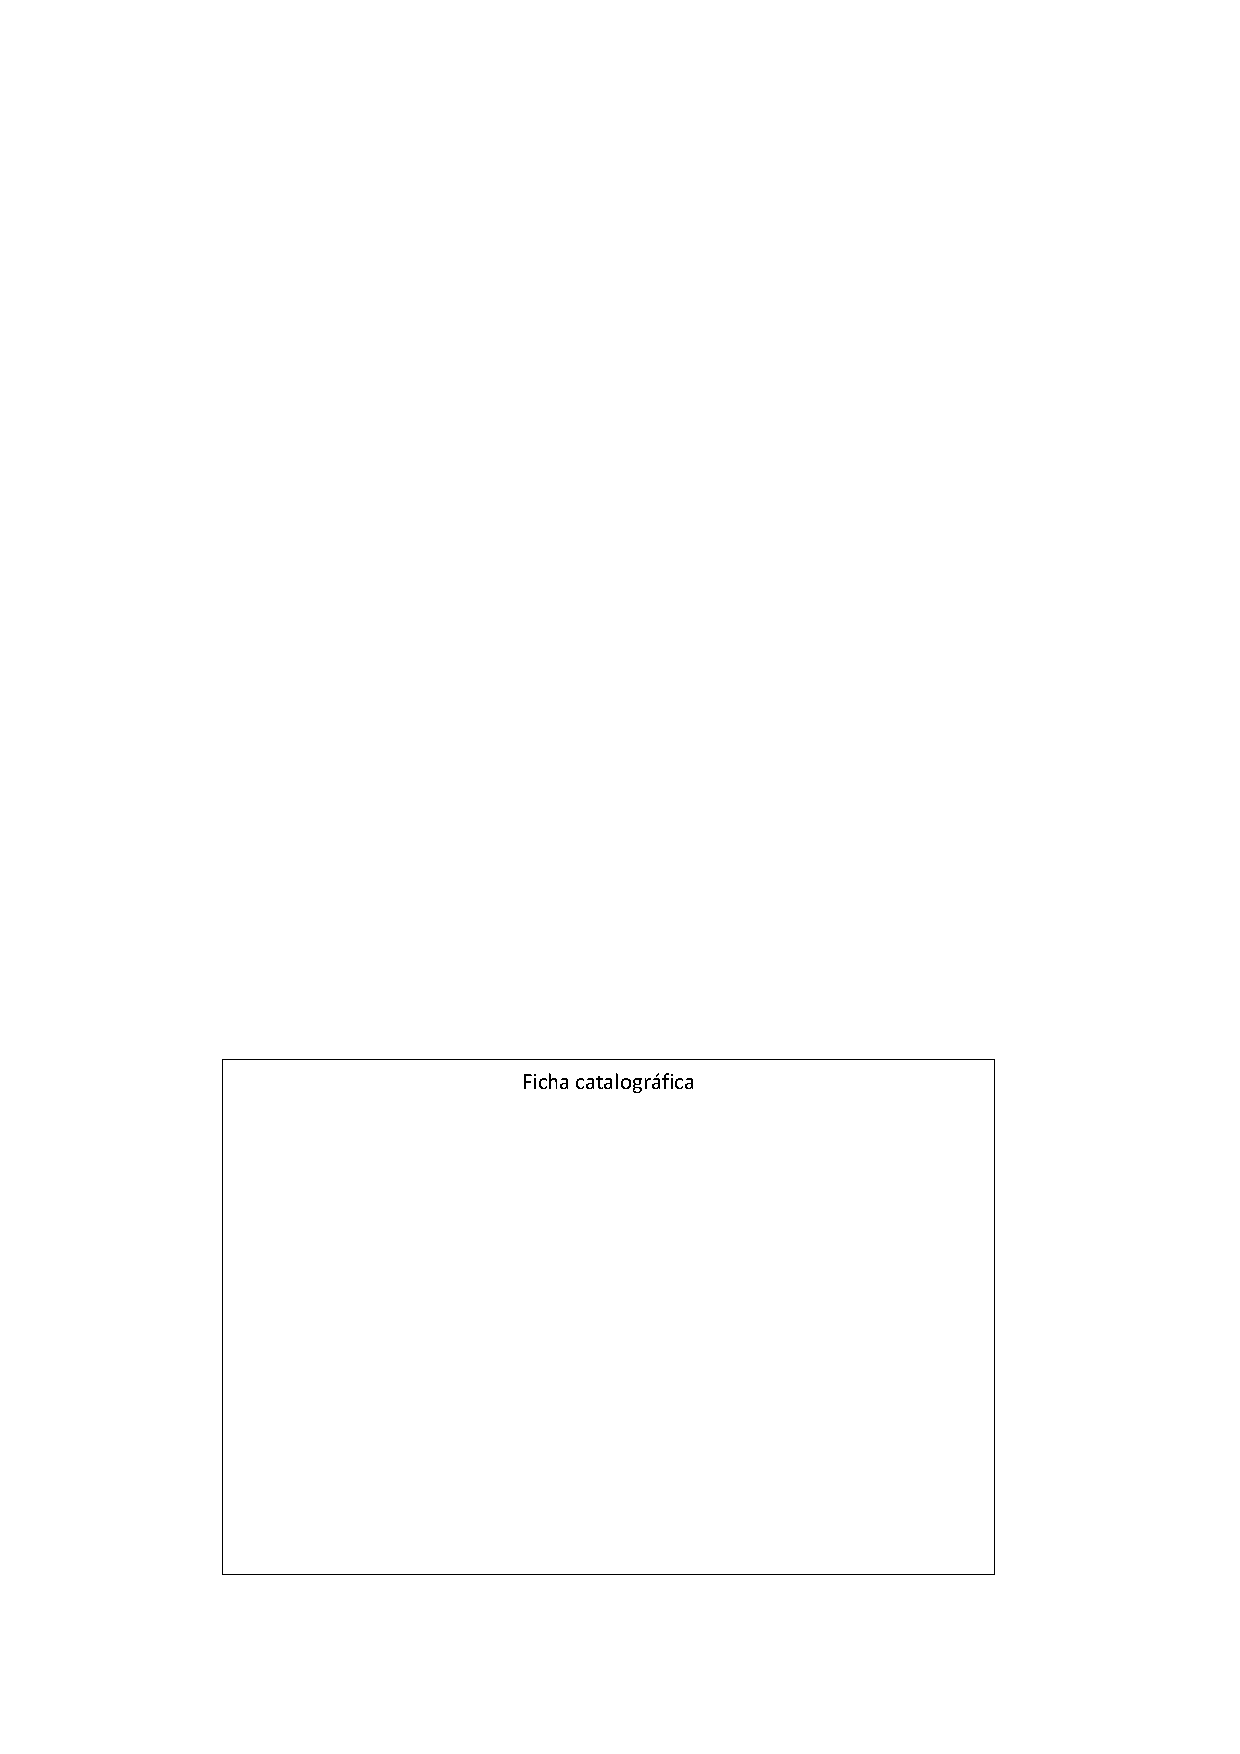
\includepdf{fig_ficha_catalografica.pdf}
\end{fichacatalografica}

% ---
% Inserir errata
% ---
%-------------------------------------------------------------------------
% Comentário adicional do PPgSI - Informações sobre ``Errata'':
%
% Usar esta página de errata apenas em casos de excepcionais, e apenas 
% para a versão corrigida da Dissertação. Por exemplo, quando depois de
% já depositada e publicada a versão corrigida, ainda assim verifica-se
% a necessidade de alguma correção adicional.
%
% Se precisar usar esta página, busque a forma correta (o modelo correto) 
% para fazê-lo, de acordo com a norma ABNT.
%
% Não usar esta página para versão original de Dissertação.
% Não usar esta página para Qualificação.
%
%-------------------------------------------------------------------------
%% +++
% \begin{errata}
% Elemento opcional para versão corrigida, depois de depositada.
% \end{errata}
%% +++
% ---

% ---
% Inserir folha de aprovação
% ---

\begin{folhadeaprovacao}
%-------------------------------------------------------------------------
% Comentário adicional do PPgSI - Informações sobre ``Folha da aprovação'':
%
% Para Qualificação, trocar por: Texto de Exame de Qualificação de autoria de Fulano de Tal, sob o título \textbf{``\imprimirtitulo''}, apresentado à Escola de Artes, Ciências e Humanidades da Universidade de São Paulo, como parte dos requisitos para obtenção do título de Mestre em Ciências pelo Programa de Pós-graduação em Sistemas de Informação, na área de concentração Metodologia e Técnicas da Computação, aprovado em \_\_\_ de \_\_\_\_\_\_\_\_\_\_\_\_\_\_ de \_\_\_\_\_\_ pela comissão examinadora constituída pelos doutores:
%
% Substituir ``Fulano de Tal'' pelo nome completo do autor do trabalho, com 
% apenas as iniciais em maiúsculo.
%
% Substiuir ``___ de ______________ de ______'' por: 
%     - Para versão original de Dissertação: deixar em branco, pois a data 
%       pode mudar, mesmo que ela já esteja prevista.
%     - Para versão corrigida de Dissertação: usar a data em que a defesa 
%       efetivamente ocorreu.
%
%-------------------------------------------------------------------------
%% +++
% \noindent Dissertação de autoria de Jonas Machado Miguel, sob o título \textbf{``\imprimirtitulo''}, apresentada à % Escola Politécnica da Universidade de São Paulo para obtenção do título de Bacharel em Engenharia Mecânica pelo   Departamento de Engenharia Mecânica, aprovada em \_\_\_\_\_\_\_ de \_\_\_\_\_\_\_\_\_\_\_\_\_\_\_\_\_\_\_\_\_\_ de \_\_\_\_\_\_\_\_\_\_ pela comissão julgadora constituída pelos doutores:
%% +++
\noindent Relatório preliminar de autoria de Jonas Machado Miguel, sob o título \textbf{``\imprimirtitulo''}, apresentado à Escola Politécnica da Universidade de São Paulo, como parte dos requisitos para obtenção do título de Bacharel em Engenharia Mecânica pelo Departamento de Engenharia Mecânica, aprovado em 4 de Maio de 2020 pela comissão examinadora constituída pelos doutores: 

\vspace*{3cm}

\begin{center}
%-------------------------------------------------------------------------
% Comentário adicional do PPgSI - Informações sobre ``assinaturas'':
%
% Para Qualificação e para versão original de Dissertação: deixar em 
% branco (ou seja, assim como está abaixo), pois os membros da banca podem
% mudar, mesmo que eles já estejam previstos.
% 
% Para versão corrigida de Dissertação: usar os dados dos examinadores que 
% efetivamente participaram da defesa. 
% 
% Para versão corrigida de Dissertação: em caso de ``professora'', trocar 
% por ``Profa. Dra.'' 
% 
% Para versão corrigida de Dissertação: ao colocar os nomes dos 
% examinadores, remover o sublinhado
% 
% Para versão corrigida de Dissertação: ao colocar os nomes dos 
% examinadores, usar seus nomes completos, exatamente conforme constam em 
% seus Currículos Lattes
% 
% Para versão corrigida de Dissertação: ao colocar os nomes das 
% instituições, remover o sublinhado e remover a palavra ``Instituição:''
%
% Não abreviar os nomes das instituições.
%
%-------------------------------------------------------------------------
\_\_\_\_\_\_\_\_\_\_\_\_\_\_\_\_\_\_\_\_\_\_\_\_\_\_\_\_\_\_\_\_\_\_\_\_\_\_\_\_\_\_\_\_\_\_\_\_\_\_\_\_\_\_\_\_
\vspace*{0.2cm} 
\\ \textbf{Prof. Dr. Fábio Gagliardi Cozman}
\\ \vspace*{0.2cm} 
Instituição: Escola Politécnica da Universidade de São Paulo
\\ \vspace*{0.2cm}
Presidente 

\vspace*{2cm}

\_\_\_\_\_\_\_\_\_\_\_\_\_\_\_\_\_\_\_\_\_\_\_\_\_\_\_\_\_\_\_\_\_\_\_\_\_\_\_\_\_\_\_\_\_\_\_\_\_\_\_\_\_\_\_\_
\vspace*{0.2cm} 
\\ \textbf{Dr. Alexandre Cristovão Maiorano} 
\\ \vspace*{0.2cm} 
Instituição: Itaú Unibanco

\vspace*{2cm}

\end{center}
  
\end{folhadeaprovacao}
% ---

% ---
% Dedicatória
% ---
%-------------------------------------------------------------------------
% Comentário adicional do PPgSI - Informações sobre ``Dedicatória'': 
%
% Opcional para Dissertação.
% Não sugerido para Qualificação.
% 
%-------------------------------------------------------------------------
\begin{dedicatoria}
   \vspace*{\fill}
   \centering
   \noindent
   \textit{To my parents, Marcionete and Pedro, for their love and courage.} 
	 \vspace*{\fill}
\end{dedicatoria}
% ---

% ---
% Agradecimentos
% ---
%-------------------------------------------------------------------------
% Comentário adicional do PPgSI - Informações sobre ``Agradecimentos'': 
%
% Opcional para Dissertação.
% Não sugerido para Qualificação.
% 
% Lembrar de agradecer agências de fomento e outras instituições similares.
%
%-------------------------------------------------------------------------
%% +++
% \begin{agradecimentos}
% \end{agradecimentos}
%% +++
% ---

% ---
% Epígrafe
% ---
%-------------------------------------------------------------------------
% Comentário adicional do PPgSI - Informações sobre ``Epígrafe'': 
%
% Opcional para Dissertação.
% Não sugerido para Qualificação.
% 
%-------------------------------------------------------------------------
%% +++
% \begin{epigrafe}
%     \vspace*{\fill}
%	\begin{flushright}
%		\textit{``Escreva aqui uma epígrafe, se desejar, ou remova esta página...''\\
%		(Autor da epígrafe)}
%	\end{flushright}
%\end{epigrafe}
%% +++
% ---

% ---
% RESUMOS
% ---

% resumo em português
\setlength{\absparsep}{18pt} % ajusta o espaçamento dos parágrafos do resumo
\begin{resumo}

%-------------------------------------------------------------------------
% Comentário adicional do PPgSI - Informações sobre ``referência'':
% 
% Troque os seguintes campos pelos dados de sua Dissertação (mantendo a 
% formatação e pontuação):
%   - SOBRENOME
%   - Nome1
%   - Nome2
%   - Nome3
%   - Título do trabalho: subtítulo do trabalho
%   - AnoDeDefesa
%
% Mantenha todas as demais informações exatamente como estão.
% 
% [Não usar essas informações de ``referência'' para Qualificação]
%
%-------------------------------------------------------------------------
%% +++
%\begin{flushleft}
%MIGUEL, Jonas Machado. \textbf{\imprimirtitulo}. \imprimirdata. \pageref{LastPage} f. %Trabalho de Conclusão de Curso (Bacharel em Engenharia Mecânica) – Escola Politécnica, %Universidade de São Paulo, São Paulo, 2020.
%\end{flushleft}
%% +++

Predizer o comportamento de sistemas regidos por correlações temporais e espaciais é uma tarefa a que se tem atribuída crescente importância em diversas áreas de aplicação, desde neurociência, epidemiologia e criminologia a logística e transporte.
Neste trabalho, delineamos o estado da arte para métodos de predição espaço-temporal e implementamos uma seleção desses métodos para a predição de geração de energia eólica no nível distrital na Alemanha.
Na análise, levamos em conta tanto séries temporais com resolução horária entre 2000 e 2015, como também especificações de projeto e de instalação de turbinas eólicas individuais.
Os modelos são avaliados em períodos não modelados e comparados com métodos convencionais de previsão. 

Palavras-chaves: Análise de Séries Temporais, Previsão Espaço-Temporal, Aprendizagem de Máquina, Redes Neurais, Energias Renováveis, Energia Eólica.
\end{resumo}

% resumo em inglês
%-------------------------------------------------------------------------
% Comentário adicional do PPgSI - Informações sobre ``resumo em inglês''
% 
% Caso a Qualificação ou a Dissertação inteira seja elaborada no idioma inglês, 
% então o ``Abstract'' vem antes do ``Resumo''.
% 
%-------------------------------------------------------------------------
\begin{resumo}[Abstract]
\begin{otherlanguage*}{english}

%-------------------------------------------------------------------------
% Comentário adicional do PPgSI - Informações sobre ``referência em inglês''
% 
% Troque os seguintes campos pelos dados de sua Dissertação (mantendo a 
% formatação e pontuação):
%     - SURNAME
%     - FirstName1
%     - MiddleName1
%     - MiddleName2
%     - Work title: work subtitle
%     - DefenseYear (Ano de Defesa)
%
% Mantenha todas as demais informações exatamente como estão.
%
% [Não usar essas informações de ``referência'' para Qualificação]
%
%-------------------------------------------------------------------------
%% +++
%\begin{flushleft}
%SURNAME, FirstName MiddleName1 MiddleName2. \textbf{Work title}: work subtitle. %\imprimirdata. \pageref{LastPage} p. Dissertation (Master of Science) – School of %Arts, Sciences and Humanities, University of São Paulo, São Paulo, DefenseYear. 
%\end{flushleft}
%% +++
Forecasting the behavior of systems in which both temporal and spatial dependencies play a central role has received increased attention, with applications domains including neuroscience, epidemiology, criminology and transportation. We review the state-of-the-art for spatio-temporal forecasting methods and implement selected approaches for predicting wind power generation at the district-level in Germany. Besides hourly time series for power generation in individual districts in 2000-2015, the analysis considers design and installation specifications for single wind turbines. The models are evaluated on unmodelled periods and locations and benchmarked against conventional forecasting methods.

Keywords: Time Series Analysis. Spatio-Temporal Forecasting. Machine Learning, Neural Networks, Wind Power.
\end{otherlanguage*}
\end{resumo}

% ---
% ---
% inserir lista de figuras
% ---
\pdfbookmark[0]{\listfigurename}{lof}
\listoffigures*
\cleardoublepage
% ---

% ---
% inserir lista de tabelas
% ---http://www2.poli.usp.br/bibliotecas/servicos/catalogacao-na-publicacao.html
\pdfbookmark[0]{\listtablename}{lot}
\listoftables*
\cleardoublepage
% ---

% ---
% inserir lista de abreviaturas e siglas
% ---
%-------------------------------------------------------------------------
% Comentário adicional do PPgSI - Informações sobre ``Lista de abreviaturas 
% e siglas'': 
%
% Opcional.
% Uma vez que se deseja usar, é necessário manter padrão e consistência no
% trabalho inteiro.
% Se usar: inserir em ordem alfabética.
%
%-------------------------------------------------------------------------
% +++
\begin{siglas}
  \item[AR] Auto-Regressive
  \item[ARIMA] Auto-Regressive Integrated Moving Average
  \item[CNN] Convolutional Neural Network
  \item[ES] Exponential Smoothing
  \item[ML] Machine Learning
  \item[PDF] Probability Density Function
  \item[PMF] Probability Mass Function
  \item[RNN] Recurrent Neural Network
  \item[ST] Spatio-Temporal
  \item[TS] Time Series
  \item[VARIMA] Vector Auto-Regressive Integrated Moving Average
  \item[VES] Vector Exponential Smoothing
\end{siglas}
% +++
% ---

% ---
% inserir lista de símbolos
% ---
%-------------------------------------------------------------------------
% Comentário adicional do PPgSI - Informações sobre ``Lista de símbolos'': 
%
% Opcional.
% Uma vez que se deseja usar, é necessário manter padrão e consistência no
% trabalho inteiro.
% Se usar: inserir na ordem em que aparece no texto.
% 
%-------------------------------------------------------------------------
% +++
\begin{simbolos}
    \item[$ \Lambda $] Lambda
\end{simbolos}
% ---

% ---
% inserir o sumario
% ---
\pdfbookmark[0]{\contentsname}{toc}
\tableofcontents*
\cleardoublepage
% ---



% ----------------------------------------------------------
% ELEMENTOS TEXTUAIS
% ----------------------------------------------------------
\textual



%-------------------------------------------------------------------------
% Comentário adicional do PPgSI - Informações sobre ``títulos de seções''
% 
% Para todos os títulos (seções, subseções, tabelas, ilustrações, etc):
%
% Em maiúscula apenas a primeira letra da sentença (do título), exceto 
% nomes próprios, geográficos, institucionais ou Programas ou Projetos ou
% siglas, os quais podem ter letras em maiúscula também.
%
%-------------------------------------------------------------------------
\chapter{Introduction}
Phenomena presenting high socio-economical relevance which are governed by complex dependencies of both spatial and temporal nature are found in diverse domains such as epidemiology, criminology, transportation, climate science and astrophysics \cite{atluri2018survey}.
Indeed, the ability to describe a system's behavior is most valuable on instances downstream in the arrow of time: forecasting \cite{armstrong2001principles, gartner2017analytics}.
Accurate, scalable and feasible rule-based forecasting modeling, however, remains elusive in many cases.
Especially as ubiquitous and continuous monitoring data become available, data-driven approaches emerge as a promising alternative.

Conventional data-driven approaches alone, however, have often shown to add limited value in spatio-temporal forecasting \cite{makridakis2018statistical}.
A major reason for this limitation lies on the assumptions they rely upon being typically violated in spatio-temporal settings.
Seasonality and spatial independency underlie most of the approaches from time series analysis, while earlier machine learning methods assume data instances are independent and identically distributed (i.i.d.) \cite{atluri2018survey}.
Recently, deep learning-based approaches have shown to be able to overcome this essentially by (a) modelling both spatial and temporal dependencies and (b) considering spatial similarities in terms less obvious than geographical proximity alone \cite{liu2017dcrnn, yao2018deep, li2019stgcn, zhang2019graphwavenet}.

In the context of renewables, accurately estimating power generation ahead of time poses a major obstacle in progressing towards carbon neutrality in power generation.
Heavily conditioned on weather and climate, harvesting energy from renewable sources is characterized by intermittency.
In the case of onshore wind power generation, climate change further aggravates this character, as wind speeds variability are expected to increase \cite{moemken2018future}.
Not accurately knowing how much wind power will be harvested in a certain time and region means power providers have to rely on unnecessarily large safety margins provided by conventional power plants for ensuring sufficient power supply.  
This ultimately hampers the expansion of wind farms and represents therefore a loss for the society, as part of the paid overall generated power is lost, as well as for the environment, as less environment-friendly power sources have to be relied upon \cite{delarue2015intermittency}.
For countries committed to large-scale initiatives such as the \textit{Energiewende} in Germany, this poses a major hindrance in decreasing overall carbon footprint in a sustainable fashion.
Accuracy on wind power generation forecasting hence has significant impact on both socio-economical and environmental aspects, in both short and long terms.

For a given installed capacity, wind power generation depends primarily on local wind speeds, which heavily vary in both time and space.
While the power generation can be predicted for each single region independently using historical data, we hypothesize that a significant increase in forecasting accuracy might be achieved by also considering inter-regional spatial dependencies. 

The objective of this work is twofold.
First, we delineate the state-of-the-art approaches for spatio-temporal forecasting in different domains.
Second, we apply selected approaches for forecasting wind power generation at the district-level in Germany.
By benchmarking against conventional approaches and single-regions forecasting horizons, we investigate whether more sophisticated modelling approaches add significant value in terms of accuracy in the use case of onshore wind power generation.  
\chapter{Background}
In this chapter, we first present the different settings, approaches, and performance metrics used in general spatio-temporal forecasting problems.
We then describe fundamental aspects of wind power generation underlying this work.

\section{Spatio-Temporal Forecasting}
In this section, we present the spatio-temporal forecasting problem, how it is approached, and how forecasting models can be assessed and compared.

\subsection{Problem statement}
In this work, we categorize spatio-temporal forecasting problems according to (1) the degree of dependency among sensors and (2) the stationarity of sensors locations.
The term sensor is used here in the abstract sense of a stochastic data generation process, which could be physically represented by an actual sensor measuring a variable of interest in a particular phenomenon.

% Problem statement for the most reduced/simplest ST forecasting setting (1), to the most general/complex one (2).
In a first regime, referred here as regime I, sensors are fixed in space, with negligible dependencies among them.
The uncertainty about the state of a sensor cannot be reduced by knowing the states of its neighboring sensors.
As a consequence, using a single model to represent the different sensors is expected to present no advantage over modeling every sensor independently.
Characteristic of this regime is also the covariance matrix for the different sensors being both diagonal and invariant in time. 

In regime II, sensors are also fixed in space, but this time with significant dependencies among them.
The uncertainty about the state of a sensor can be reduced by knowing the states of its neighboring sensors.
In other words, uncertainties among sensors are coupled.
Modeling sensors together could be potentially beneficial in such case. 
Besides, the covariance matrix is expected to be non-diagonal but still invariant in time. 

Finally, in regime III, dependent sensors move in space.
Dependencies across sensors should hence also change over time, and a corresponding time-dependent covariance matrix is expected to follow. 
Again, models representing multiple sensors could make use of this and outperform models for single sensors. 

\subsection{Conventional Approaches}
In this work, we refer as conventional approaches what is in the literature often referred as Time Series \footnote{A time series is defined as a stochastic process ${..., X_{t-1}, X_{t}, X_{t+1}, ...}$ consisting of random variables indexed by time index $t$. The stochastic behavior ${X_t}$ is described by $p(x_{t1}, x_{t2}, ..., x_{tm})$, i.e.,the PDF (or PMF) for all finite collections of time indexes ${(t_1, t_2, ..., t_m), m<\infty}$ \cite{kempthorne2013s0196}. } approaches.
Their formulations were motivated by forecasting problems in which time was the single independent variable.
The hallmark of conventional forecasting approaches is their reliance on the well-developed theory for describing stationary random processes. 
There are two general ways of describing (modeling) a generic time series: (1) the Exponential Smoothing (ES) framework, and (2) the Auto-Regressive Integrated Moving Average (ARIMA) framework \cite{brockwell1991methods}. 

\subsubsection{Exponential Smoothing Framework}
In the ES framework, time series are modelled as a superposition of three components: trend ($m_t$), seasonal ($s_t$), and random noise ($Y_t$).
This is known as the Classical Decomposition (\autoref{classical-decomposition}).

\begin{equation}\label{classical-decomposition}
    X_t = m_t + s_t + Y_t
\end{equation}

The underlying principle is to apply a filter to $X_t$ that smooths out the noise component $Y_t$, allowing $m_t$ and $s_t$ to be estimated and extracted.
Techniques within this framework differ by (a) the filter, (b) the assumptions on and preprocessing of $X_t$. 
In fact, the simplicity of models based on ES and their success in temporal forecasting problems have made this framework the default choice in the industry for such settings \cite{holt2004forecasting}.
We describe two methods as examples: (1) the least squares, (2) the exponential smoothing method.
Both assume non-seasonality of $X_t$ (i.e.,$s_t=0$), meaning a deseasoning of the time series is typically required as a preprocessing step.

In the least squares method, $m_t$ is first approximated by a parametric family of functions (e.g. $m_t = a_0 + a_1 t + a_2 t^2$).
The parameters are then estimated via the the minimization of the squared errors $\Sigma_t (x_t - m_t)^2$. 

In the exponential smoothing method, a pre-defined $a \in [0, 1]$ is used for the estimated trend $\hat{m}_t$ by \autoref{exponential-smoothing}.
\begin{align}\label{exponential-smoothing}
    \hat{m}_t &= a X_t + (1-a) \hat{m}_{t-1}, t=1, ..., n
    \hat{m}_1 &= X_1
\end{align}

The resulting expression of $\hat{m}_t$ in terms of the past measurements $X_t, X_{t-1}, ...$, motivates the name of this method:
\begin{equation}\label{exponential-smoothing2}
    \hat{m}_t = \sum_{j=0}{t-2} a (1-a)^j X_{t-j} + (1-a)^{t-1} X_1 \hat{m}_{t-1}, 
\end{equation}
i.e.,$\hat{m}_t$ is a weighted moving average of the past measurements $X_t, X_{t-1}, ...$, with weigths decreasing exponentially.

So far, the exponential smoothing framework has been presented in its univariate version.
Its multivariate version is the Vector Exponential Smoothing (VES) framework.  
While ES-based models can be used to properly address regime I forecasting problems, VES-based models can incorporate cross-sensors dependencies into the covariance matrix to model sensors under regime I, II or III.

\subsubsection{ARIMA Framework}
% ARIMA framework (univariate version: ARIMA; multivariate VAR, VARIMA)
First proposed by \cite{box1970time} (and hence often referred as Box-Jenkins Methods), the ARIMA framework relies on differencing to achieve stationarity.
Differencing operators, are recursively applied to the data ${x_t}$ until the resulting observations are approximatelly stationary. \cite{brockwell1991methods}
For $k$ recursions, the corresponding operator is referred as $\nabla^k(\cdot)$.
As an instance, for k=1: $\nabla X_t = X_{t} - X_{t-1}$.

The framework is named after the ARIMA model, described by \autoref{arima}, with the autoregressive operator $\phi_k$, moving average operator $\theta_k$ (both of order $k$), and innovation (white noise) at time index $t$ $a_t$.
\begin{align}\label{arima}
    x_t = & \phi_1 x_t + ... + \phi_{p+d} x_{t-p-d}
          & - \theta_{1} a_{t-1} - ... - \theta{q} a_{t-q} + a_t 
\end{align}
The first line of \autoref{arima} corresponds to the autoregressive (AR) component of ARIMA, in which $x_t$ is represented as a linear regression of its preceding values $x_{t-1}, ..., x_{t-p-d}$.

Important nonlinear methods are included in this framework, such as ARCH and GARCH, in which the innovation term is modelled by respectively by an AR model and by an ARMA model.
The multivariate version of ARIMA is the Vector-ARIMA (VARIMA).
Like its counterpart from the Exponential Smoothing, VARIMA models make use of a covariance matrix to incorporate cross-sensors dependencies for the higher coupling regimes II and III.

\subsection{Machine Learning-based Approaches}
Machine Learning approaches rely on (1) definition of relatively general architectures and (2) finding a configuration of parameter values in the given architecture that minimizes the expectation of some loss function.
As the loss function represents a discrepancy between predictions and ground truth, this optimization process leads to a model that can be used to predict system behavior given a configuration for inputs values.
The optimization process itself is typically performed by a gradient-based algorithm. \cite{goodfellow2016deep}

In the context of univariate temporal forecasting (i.e.,regime I), the performance of Machine Learning algorithms was considered by some to be very limited reliability and usefulness \cite{makridakis2000m3}.
However, \cite{bengio2019nbeats} recently demonstrated that a "pure" Deep Learning approach could not only (1) consistently outperform conventional ones, but also (2) be less reliant on manual tuning and (3) be made interpretable in both final and intermediate outputs.
Until then, top-performing ML-based models were either a result of a combination or hybridization with conventional methods.
Earlier approaches relied on ML-TS Combinations, in which outputs from statistical engines were used as features for ML algorithms.
Later, TS models had their parameters optimized via gradient-descent and stacked with a Recurrent Neural Network (RNN) to form a hybrid model \cite{smyl2020esrnn}.

Outside of regime I, ST forecasting problems were already successfully addressed by Deep Learning approaches, such as in forecasting traffic \cite{liu2017dcrnn}, ride-hailing demand \cite{li2019stgcn} and electrical power demand \cite{toubeau2018blstm}.
Most of these approaches relied on RNN architectures, eventually combined with a CNN architecture.
More recently, approaches that model the Spatio-Temporal dependencies over a non-Euclidean space in a graph representation have been proposed and currently represent the state-of-the-art for ST forecasting problems \cite{zhang2019graphwavenet}.

\subsection{Forecasting Performance Metrics}
Different quantities can be used for assessing models forecasting performance.
Some of the most popular are $MAE$ (Mean Absolute Error, \autoref{mae}), $MAPE$ (Mean Absolute Percentual Error, \autoref{mape}), $RMSE$ (Root Mean Squared Error, \autoref{rmse}).
As they expose different qualities of performance, combining a reasonable number of metrics can be advisable.  
\begin{equation}\label{mae}
    MAE(\bm{\hat{X}}^{(t+i):(t+T)}; \bm{\Theta}) = \frac{1}{T N D} \Sigma_{i=1}^{T} \Sigma_{j=1}^{N} \Sigma_{k=1}^{D} | \bm{\hat{X}}^{(t+i)}_{jk} - X_{jk}^{(t+i)} |
\end{equation}

\begin{equation}\label{mape}
    MAPE(\bm{\hat{X}}^{(t+i):(t+T)}; \bm{\Theta}) = \frac{100}{T N D} \Sigma_{i=1}^{T} \Sigma_{j=1}^{N} \Sigma_{k=1}^{D} \frac{ | \bm{\hat{X}}^{(t+i)}_{jk} - X_{jk}^{(t+i)} | }{ |X_{jk}^{t+i}| }
\end{equation}

\begin{equation}\label{rmse}
    RMSE(\bm{\hat{X}}^{(t+i):(t+T)}; \bm{\Theta}) = \sqrt{ \frac{1}{T N D} \Sigma_{i=1}^{T} \Sigma_{j=1}^{N} \Sigma_{k=1}^{D} (\bm{\hat{X}}^{(t+i)}_{jk} - X_{jk}^{(t+i)})^2 }
\end{equation}


\section{Wind Power Generation}
% Wind power: variables affecting available energy
% Wind power: variables affecting conversion of (part of) available energy effective generated power
% Economics (costs)
% Economics (market)
% key parameters in wind power generation (capacity factor), intermittent nature & why forecasting is important (potential)
% Power generation measurements in a single turbine, as well as its aggregation by farm or by district as a stochastic process
% This stochastic process can be cast as a Time Series
\chapter{Use Case}

\section{Requirements}
\section{Resources}
\subsection{Dataset}
\input{04_Pipeline-Concept}
\input{05_Pipeline-Development}
\input{06_Results-and-Discussion}
\input{07_Conclusion-and-Overlook}

% ----------------------------------------------------------
% ELEMENTOS PÓS-TEXTUAIS
% ----------------------------------------------------------
\postextual
% ----------------------------------------------------------

% ----------------------------------------------------------
% Referências bibliográficas
% ----------------------------------------------------------
\bibliography{referencias}

% ----------------------------------------------------------
% Glossário
% ----------------------------------------------------------
%
% Consulte o manual da classe abntex2 para orientações sobre o glossário.
%
%\glossary

% ----------------------------------------------------------
% Apêndices
% ----------------------------------------------------------

% ---
% Inicia os apêndices
% ---
\begin{apendicesenv}

% Imprime uma página indicando o início dos apêndices
%\partapendices

%-------------------------------------------------------------------------
% Comentário adicional do PPgSI - Informações sobre ``apêndice''
%
% Para todos os captions/(títulos) (de seções, subseções, tabelas, 
% ilustrações, etc):
%     - em maiúscula apenas a primeira letra da sentença (do título), 
%       exceto nomes próprios, geográficos, institucionais ou Programas ou
%       Projetos ou siglas, os quais podem ter letras em maiúscula também.
%
% Todas  as tabelas, ilustrações (figuras, quadros, gráficos, etc. ), 
% anexos, apêndices devem obrigatoriamente ser citados no texto.
%      - a citação deve vir sempre antes da primeira vez em que a tabela, 
%        ilustração, etc., aparecer pela primeira vez.
%
%-------------------------------------------------------------------------

\end{apendicesenv}
% ---


% ----------------------------------------------------------
% Anexos
% ----------------------------------------------------------

% ---
% Inicia os anexos
% ---
\begin{anexosenv}

\end{anexosenv}

%---------------------------------------------------------------------
% INDICE REMISSIVO
%---------------------------------------------------------------------
%%%%%MF\phantompart
%%%%%MF\printindex
%---------------------------------------------------------------------

\end{document}
